\section{The process of budgeting}
\begin{itemize}
    \item Planning is not a simple job when it comes to time, similarly it is complicated when it comes to cost.
    \item Budgeting seeks to answer questions such as:
        \begin{itemize}
            \item What financial resources do they need to create the deliverables?
            \item Are there going to be additional expenses?
            \item Will they need the money?
            \item Where will it come from?
            \item What is the total budget?
            \item Who will control the costs? how?
        \end{itemize}
    
    \item The most convinient way of answering these questions is the task of te project budget list.
    \item Building the project budget list follows a similar structure to building a project schedule. Here are the steps:
        \begin{enumerate}
            \item Identify the activities that cost money from your work breakdown structure or activity list.
            \item Estimate the cost of each work package, task and deliverable.
            \item Add buffers and account for uncertainties.
            \item You should be ready to time the expenses that can be done using a gantt chart.
            \item Put it all together into a project budget.
        \end{enumerate}
    
    \item Remember the optimism bias, just like in planning time humans often underestimate the time taken, humans tend to underestimate cost too.
    \item The PM needs to be accurate and avoid the optimism bias.
\end{itemize}

%%%%%%%%%%%%%%%%%%%%%%%%%%%%%%%%%%%%%%%%%%%%%%%%%%%%%%
\section{The process of budgeting (continued)}
\begin{itemize}
    \item The first step of cost planning is identifying all the cost generating activites.
    \item You need to get your work breakdown structure and activity list. Using the activity list check for potential costs that will not be covered by the company, these cost will be most likely covered by someone else, such as another company that we hired to do certain jobs such as paint walls and such. Who will buy the paint? us or the painting company? This all needs to be agreed upon before anything starts and it must be mentioned and agreed upon in a contract.
    \item You need the project sponsr to advise how to factor the cost. Communicating with the appropriate people is crucial.
    \item You need to be in contact with HR for hiring and answering questions such as the following: 
        \begin{itemize}
            \item How many staff members are needed?
            \item What jobs they will have?
            \item What costs will be incurred for recruitment?
            \item Who will train the new hires? You or another company?
            \item Will they be interviewed on site or in an external center?
        \end{itemize}
    
    \item If you have built a detailed and extensive activity list them identifying which ones incur costs should be a lot easier. Budget planning may make you aware of tasks that you did not factor into the project schedule.
    \item Now that we have a list of all the costs, it is time to estimate what those costs will be. Some tasks will be straight forward to estimate but others will not, some will require negotiation with other comapanies, others will require contacting many people and negotiating.
    \item Using information from past projects is a very useful tactic. 
    \item Take into account the optimism bias and adding buffers.
    \item Track all the costs and spending in a project budget sheet.
        \begin{figure}[H]
            \centering
            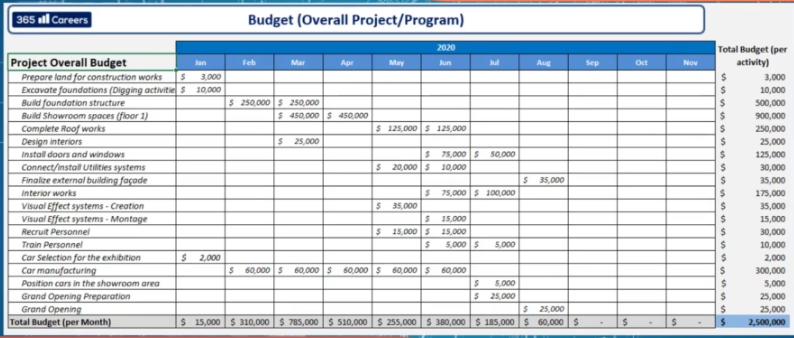
\includegraphics[width=\width\textwidth]{./figs/20221027103732.png}
            %\caption{}
        \end{figure}
\end{itemize}

%%%%%%%%%%%%%%%%%%%%%%%%%%%%%%%%%%%%%%%%%%%%%%%%%%%%%%
\section{Procurement contract types}
\begin{itemize}
    \item It is often the case that the company will not have the resources they need for a project, so a PM must look elswhere for the resources. 
    \item The PM needs to be aware of the timelines, due dates and the quality levels of all resources expended and estimated.
    \item There are three types of contracts a PM can use for this.
\end{itemize}

\subsection{3 contracts}
\begin{itemize}
    \item Fixed price: The vendor commits to doing the work for a set of amount within a certain timeframe.
        \begin{itemize}
            \item Pro: any additional spending will be taken on by the vendor, no risk for us.
            \item Con: Before signing the contract, they will most likely put a big buffer in the initial price. Or if costs do get too high they might decrease the scope or the quality in order to compensate.
            \item This beneficial to use when the scope is clear to all parties. 
        \end{itemize}
    
    \item Cost plus contract:
        \begin{itemize}
            \item The buyer agrees to pay any cost incurred by the vendor performing the work. 
            \item This can be a variable fee, a fixed additional fee or a mix.
            \item The risks here is that the buyer incurs all of the extra costs, the vendor can also keep working longer than needed or adding extra items to the 'to-do list'.
            \item This contract makes sense if the scope is not easy to define, but controls must be put in place in order to avoid over spending in non-essential things for the project. 
        \end{itemize}
    
    \item Time and materials contract:
        \begin{itemize}
            \item It's a mix of the fixed price and cost plus.
            \item The vendor charges the buyer a hourly or daily rate.
            \item This is a good option when the scope is not clear and the work is more labor based than material based. 
            \item Similar risk to the cost plus contract, thus set controls to avoid the risks (overspending in non-essential things).
        \end{itemize}
\end{itemize}

\subsection{Conclusion}
\begin{itemize}
    \item There are many variations that can be tailor-made.
    \item You can even include inflation if the project spans a long time.
    \item You can add or decrease incentives as needed.
    \item The PM must have a good understanding of all risks and benefits that each agreement can have. 
\end{itemize}

%%%%%%%%%%%%%%%%%%%%%%%%%%%%%%%%%%%%%%%%%%%%%%%%%%%%%%
\section{Procuring non-financial resources}
\begin{itemize}
    \item It's not all about the money in PM.
    \item Non-financial resources, which is to say humans, are also needed.
    \item Now for another analysis.
\end{itemize}

\subsection{Analysing non-financial resources}
It has four parts:
\begin{enumerate}
    \item Define the type of resource:
        \begin{itemize}
            \item Take your work breakdown structure and see what expertise you need, if the expertise can be found within the organization or extra hiring will be required.
            \item Also allocate time to check management availability, if something needs to check something, do not assume they are always available, allocate some days for them to get to it. They are busy people.
        \end{itemize}

    \item Estimate how much time you will need.
        \begin{itemize}
            \item Estimate the time each expert will need to complete the activities.
            \item Take into account the optimism bias and adding buffers.
        \end{itemize}
        
    \item Validate the availability of the people you need.
        \begin{itemize}
            \item (From next lecture: Planning HR)
            \item You need to check when the experts can give you their time. 
            \item You can make a schedule with the person who needs to complete the activities and by when.
            \item Its important to keep track of employee schedule. And be in constant contact with the department heads, because sometimes they already have other activities and cannot give you any time, or refuse you access to them for any reason. If this is the case, you will need to work out a new plan with the project sponsor. 
            \item Also very important: don't forget to check their personal availability such as vacations, holidays, etc.
            \item Creating a schedule looks like this:
                \begin{figure}[H]
                    \centering
                    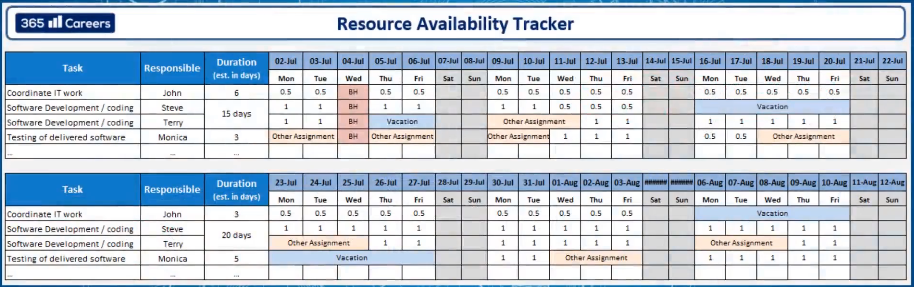
\includegraphics[width=\width\textwidth]{./figs/20221027110425.png}
                    %\caption{}
                \end{figure}
                \begin{itemize}
                    \item List the tasks in a column, then who is responsable for them, the duration. Then a calendar with all the marked vacations, holidays, and non-availability days.
                \end{itemize}
        \end{itemize}
    
    \item Assign roles and responsabilities to them
        \begin{itemize}
            \item (From next lecture: RACI matrix - assigning roles)
            \item To assign roles and responsabilities we can use several tools, the first one is a simple list:
                \begin{figure}[H]
                    \centering
                    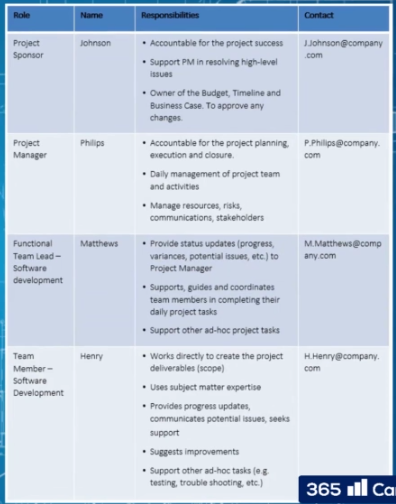
\includegraphics[width=\width\textwidth]{./figs/20221027110819.png}
                    %\caption{}
                \end{figure}
                \begin{itemize}
                    \item It just has the role, name and responsability along with the contact info.
                    \item This is a people oriented document that is high level and simplified.
                \end{itemize}
            
            \item The second tool is the RACI matrix:
                \begin{figure}[H]
                    \centering
                    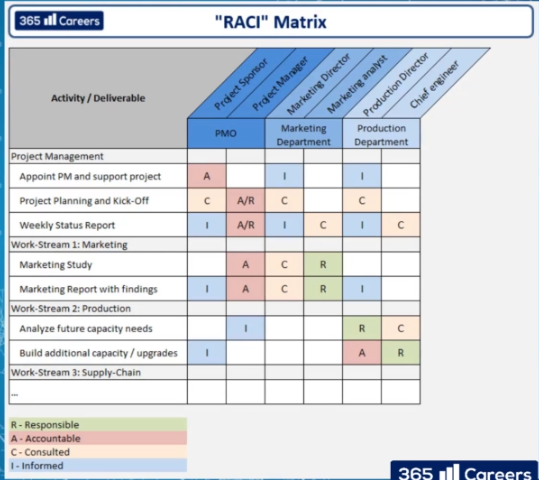
\includegraphics[width=\width\textwidth]{./figs/20221027110929.png}
                    %\caption{}
                \end{figure}
                \begin{itemize}
                    \item Each letter of RACI stands for something.
                    \item R: responsable, the person who is directly responsable for doing the work.
                    \item A: accountable, the person resonsable for meeting the overall goal of the activity.
                    \item C: consulted, the person who provides information expertise or support for an activity.
                    \item I: informed: the person who needs to be informed on the status of an activity.
                    \item For most of the activities the PM will be accountable.
                    \item This is a lower level document compared to the simple list since more details are included and it is more formal. This is task oriented.
                \end{itemize}
            
            \item The PM must choose which tool to use either one or the other or a mix of both.
        \end{itemize}
\end{enumerate}

%%%%%%%%%%%%%%%%%%%%%%%%%%%%%%%%%%%%%%%%%%%%%%%%%%%%%%
\section{Quality requirements}
\begin{itemize}
    \item Quality: the standard of something as measured against other things of a similar kind. The degree of excellence of something.
    \item In PM quality means: the quanlitative characteristics of a product, either phisical qualities, performance or service related.
    \item The PM needs to work with stakeholders to ensure that quality standards are being met on the deliverables.
    \item There is a five step process:
        \begin{enumerate}
            \item Defne the quality standards and requirements (could be according to laws or regulations too).
                \begin{itemize}
                    \item The PM needs to ensure standards are met.
                    \item Depending on the project, we might need to outsource or work with other companies for the quality assurance aspect. This is not a straight forward path since there is negotiating and constant issues that need to be spoted and corrected.
                \end{itemize}

            \item Setting the actual, and actionable, targets for the criteria.
                \begin{itemize}
                    \item Set goals like: producing product with less of 0.5\% defects. 
                    \item Setting a tolerance level and using statistical methods helps ensure the quality goals are being actually met.
                    \item When it comes to services we need to set similar goal measuring metrics such as in a call center: less tha 5\% calls lost per month, or over 98\% of incidents solved.
                \end{itemize}
            
            \item Plan how, when and who will measure quality.
                \begin{itemize}
                    \item The PM must appoint someone to measure, and also must have clear what metrics we will use (as indicated in the previous step).
                    \item The PM must audit the quality assurance to check wether the quality assurance metrics are actually being checked and passed.
                \end{itemize}
            
            \item Finalizing the quality plan:
                \begin{itemize}
                    \item The PM collects all the information and creates yet another document, this document must include:
                        \begin{itemize}
                            \item Quality standards, target result, sample size of audits, frequency of reports, owner.
                        \end{itemize}
                \end{itemize}
            
            \item Make adjustments to their project constraints:
                \begin{itemize}
                    \item A quality plan can incrase the scope, the cost or the time for project completion in a number of ways. 
                    \item Just in case any quality checks are not passed, a PM must identify risks and put buffers for when this happens so that the product, service and project comply with standards, this might require additional time and money so we must take this planning also into account.
                \end{itemize}
        \end{enumerate}
\end{itemize}